\level{2}{Processo di sviluppo}
		\level{3}{Studio di Fattibilità}
			Lo \insdoc{Studio di Fattibilità} deve essere rapido e accurato.\\
			Il documento di \insdoc{Studio di Fattibilità} viene redatto dagli analisti, sulla base di ciò che emerge dalle prime due riunioni. Qui i membri del gruppo si confrontano su tematiche riguardanti i capitolati quali:
			\begin{itemize}
				\item il dominio applicativo e tecnologico;
				\item il rapporto costi/benefici:
				\begin{itemize}
					\item confronto tra mercato attuale e futuro;
					\item costo di produzione e redditività dell'investimento;
				\end{itemize}
				\item i rischi ai quali essi sono soggetti.
			\end{itemize}

		\level{3}{Analisi dei Requisiti}
			Durante l'\insdoc{Analisi dei Requisiti} vengono catalogati e descritti tutti i requisiti che il \insglo{prodotto} dovrà possedere. Tali requisiti sono ottenuti da una delle seguenti fonti (presentate in ordine decrescente di importanza):
			\begin{enumerate}
				\item \insglo{capitolato} d’appalto;
				\item incontri con il proponente;
				\item incontri con il committente;
				\item valutazioni interne al gruppo di lavoro.
			\end{enumerate}
			Tali requisiti sono raccolti all'interno del documento \insdoc{Analisi dei Requisiti}. All'interno di tale documento è anche indicato un modo per verificare i requisiti in esso raccolti.
			\level{4}{Norme}
				\level{5}{Classificazione dei casi d'uso} \label{sec:classificazioneUC}
					I casi d'uso vengono identificati univocamente da una sigla nella forma UCYX.
					\begin{itemize}
						\item Y può assumere tre valori: N, A o D. N rappresenta tutti i casi d'uso inerenti a \insglo{Norris}, A rappresenta quelli inerenti l'applicazione \insglo{Android} e D rappresenta quelli che riguardano la \insglo{Dashboard}.
						\item X è un codice gerarchico numerico.
					\end{itemize}
					Sarà compito degli \insrole{analisti} identificare i casi d'uso e essi dovranno preoccuparsi di fornire un diagramma conforme allo standard \insglo{UML} per ogni caso d'uso non foglia. Qui di seguito sono riportate le informazioni da inserire nella parte testuale:
					\begin{itemize}
						\item titolo;
						\item attori (principali e secondari);
						\item precondizione;
						\item postcondizione;
						\item flusso principale degli eventi, dove si descrive il flusso dei casi d'uso figli; per ogni evento va specificato quanto segue:
						\begin{itemize}
							\item descrizione testuale;
							\item attori coinvolti;
							\item se l’evento è descritto nel dettaglio da un altro caso d’uso;
						\end{itemize}
						\item scenari alternativi; per ognuno di essi va specificato quanto segue:
						\begin{itemize}
							\item descrizione testuale;
							\item attori coinvolti;
							\item se lo scenario è descritto nel dettaglio da un altro caso d’uso.
						\end{itemize}
					\end{itemize}
				\level{5}{Classificazione dei requisiti}
					I requisiti dovranno essere classificati per tipo e importanza, utilizzando la seguente codifica: R[X][Y][Z].\\
					La codifica appena presentata deve essere interpretata nel modo seguente:
					\begin{enumerate}
						\item X indica l'importanza strategica del requisito e può assumere uno dei seguenti valori:
						\begin{itemize}
							\item R: requisiti obbligatori (required);
							\item D: requisiti desiderabili (desiderable);
							\item O: requisiti opzionali (optional).
						\end{itemize}
						\item Y indica la tipologia del requisito e può assumere i seguenti valori:
						\begin{itemize}
							\item F: indica che si tratta di un requisito funzionale (functional);
							\item P: indica che si tratta di un requisito prestazionale (performance);
							\item Q: indica che si tratta di un requisito di qualità (quality);
							\item C: indica che si tratta di un requisito di vincolo (constraint).
						\end{itemize}
						\item Z indica il codice gerarchico che identifica un requisito e dev'essere univoco.
					\end{enumerate}
	\level{4}{Strumenti}
		\level{5}{Software per la creazione di diagrammi UML}
			Per l'attività di Analisi dei Requisiti sono stati utilizzati i seguenti strumenti:
			\begin{itemize}
				\item per la creazione dei diagrammi \insglo{UML} è stato utilizzato il \insglo{software} \insglo{Astah};
				\item per la classificazione dei requisiti è stata utilizzata un'applicazione web creata dagli \insrole{Amministratori}.
			\end{itemize}
			Il \insglo{software} \insglo{Astah} è descritto nell'appendice \nameref{app:strumenti}, mentre l'applicazione per la classificazione dei requisiti è descritta nell'appendice \nameref{sec:tracker}.
			
	\level{3}{Progettazione}
		Scopo dell'attività di progettazione è produrre una soluzione soddisfacente per tutti i soggetti coinvolti nel progetto, una volta compreso esattamente quali sono i requisiti del problema. \\
		Approfondendo la progettazione del \insglo{prodotto} fino ad arrivare a moduli abbastanza semplici da essere capiti da una sola persona, si otterranno le istruzioni necessarie ai \insrole{Programmatori} per ottenere il \insglo{prodotto} finito.
			
		\level{4}{Progettazione architetturale}
			Prima di procedere alla definizione vera e propria dell'architettura dei vari prodotti \insglo{software}, devono essere eseguiti e successivamente documentati i seguenti task:
			\begin{enumerate}
				\item si individuano i prodotti che si intendono realizzare;
				\item si definiscono ruoli e responsabilità di ognuno dei prodotti individuati;
				\item si definiscono le interazioni che i prodotti hanno fra di loro;
				\item ci si assicura che ogni requisito sia soddisfatto da almeno uno dei prodotti individuati e descritti;
				\item ci si assicura che ogni \insglo{prodotto} realizzi almeno un requisito.
			\end{enumerate}
			A questo punto si può procedere con la progettazione dell'architettura dei prodotti \insglo{software} che si intendono realizzare. Si devono eseguire e successivamente documentare i seguenti task per ognuno dei prodotti individuati:
			\begin{enumerate}
				\item si suddivide il \insglo{prodotto} in componenti;
				\item si definisce il ruolo di ogni componente individuato;
				\item si definiscono le interazioni che i componenti hanno fra loro;
				\item si definiscono le eventuali interfacce che ogni componente mette a disposizione dell'ambiente esterno;
				\item ci si assicura che ogni requisito sia soddisfatto da almeno uno dei componenti individuati e descritti;
				\item ci si assicura che ogni componente realizzi almeno un requisito;
				\item si realizzano e si documentano i test di integrazione, necessari per verificare il corretto funzionamento di più componenti assemblati insieme (le norme da seguire sono presenti nella sezione \nameref{sec:TestIntegrazione}).
			\end{enumerate}
			Durante la suddivisione del \insglo{prodotto} in componenti è auspicabile che i \insrole{Progettisti} utilizzino in modo appropriato i \insglo{design pattern}. Qualora ciò dovesse avvenire, si documenta la cosa procedendo con una loro descrizione e contestualizzazione (per maggiori informazioni si consulti la sezione \nameref{sec:ProgArcDesingPattern}).\\
			Un utile supporto alla documentazione di tutti i task precedentemente descritti sono i diagrammi \insglo{UML}. Per maggiori informazioni si consulti la sezione \nameref{sec:ProgArcUML}.\\
			Il modo in cui viene effettuato il tracciamento dei requisiti viene descritto in modo più approfondito nella sezione \nameref{sec:ProgTracCompReq}.
			\level{5}{Norme}
				\level{6}{Design Pattern} \label{sec:ProgArcDesingPattern}
					Al fine di consentire una migliore comprensibilità delle scelte progettuali e della progettazione stessa, i \insrole{Progettisti} dovranno indicare i \insglo{pattern} architetturali impiegati, fornendo per ciascuno di essi:
					\begin{itemize}
						\item una descrizione testuale e grafica;
						\item la motivazione che ha portato alla sua scelta;
						\item una breve descrizione dell'applicazione del \insglo{pattern} al progetto.
					\end{itemize}
				\level{6}{Diagrammi UML} \label{sec:ProgArcUML}
					La documentazione riguardante i prodotti e i componenti individuati deve sempre fare uso di diagrammi \insglo{UML}. Essi sono necessari per esplicitare e formalizzare in modo migliore i vari aspetti che sono stati descritti testualmente.\\
					In particolare, durante la progettazione architetturale è necessario fare uso dei seguenti diagrammi:
					\begin{description}
						\item[diagrammi dei componenti] Essi hanno lo scopo di rappresentare la struttura interna di un \insglo{prodotto} \insglo{software} modellato in termini dei suoi componenti principali e delle relazioni fra di essi. Questo tipo di diagramma viene dunque utilizzato per evidenziare i componenti (e le relazioni che essi hanno fra di loro) individuati all'interno di ciascun \insglo{prodotto} \insglo{software}.
						\item[diagrammi delle attività] Essi hanno lo scopo di definire le attività da svolgere per realizzare una certa funzionalità. Vengono dunque usati per mostrare come determinate interazioni tra componenti (o fra prodotti) realizzino una funzionalità che si intende rendere disponibile.
					\end{description}
					Tali diagrammi dovranno seguire le indicazioni fornite nella sezione \nameref{sec:UML}.

				\level{6}{Classificazione dei componenti} \label{sec:ClassificareComponenti}
					I componenti vengono identificati univocamente da una descrizione nella forma NomeProdotto::NomeComponente.
					\begin{itemize}
						\item NomeProdotto rappresenta il nome del \insglo{prodotto} \insglo{software} che i \insrole{Progettisti} hanno deciso di realizzare.
						\item NomeComponente rappresenta il nome che è stato dato dai \insrole{Progettisti} al componente individuato.
					\end{itemize}
					A ogni componente è inoltre associato un codice univoco nella forma XY, dove X è l'iniziale del del nome del \insglo{prodotto} e Y un numero intero crescente (che parte da 0).
				\level{6}{Test di integrazione} \label{sec:TestIntegrazione}
					Per ottenere maggior efficienza ed efficacia durante l'attività di test, è auspicabile che i \insrole{Progettisti} si preoccupino di definire delle classi di verifica per appurare che il funzionamento dei componenti sia quello previsto. Sarebbe infatti ideale poter fornire degli strumenti completamente automatici ai \insrole{Verificatori}.\\
					La progettazione delle classi per la verifica deve essere fatta da persone diverse da coloro che hanno progettato la classe da verificare, quando ciò fosse possibile.
			\level{5}{Strumenti}
				Per la progettazione architetturale sono stati utilizzati i seguenti strumenti:
				\begin{itemize}
					\item per la creazione dei diagrammi \insglo{UML} è stato utilizzato \insglo{Astah};
					\item per il tracciamento delle componenti è stata utilizzata l'applicazione web sviluppata dagli \insrole{Amministratori}.
				\end{itemize}
				Il \insglo{software} \insglo{Astah} è descritto in modo dettagliato nell'appendice \nameref{app:strumenti}, mentre l'applicazione web per il tracciamento viene descritta nell'appendice \nameref{sec:tracker}.
			\level{5}{Procedure}
				\level{6}{Tracciamento componenti-requisiti} \label{sec:ProgTracCompReq}
					È fondamentale che ogni requisito sia soddisfatto da almeno un componente. Per controllare che ciò sia vero è necessario prima di tutto effettuare il tracciamento. Si seguano i passi descritti nella seguente \insglo{procedura}. Si noti che qui si da per scontato che i componenti e i requisiti siano già stati inseriti precedentemente sul Tracker del gruppo (per l'inserimento dei componenti fare riferimento alla \insglo{procedura} descritta nella sezione \nameref{sec:InsComponente}).
					\begin{enumerate}
						\item Accedere al Kaizen \insglo{Team} Tracker (\insuri{http://kaizenteam.it/tracker/}).
						\item Entrare all'interno della sezione “Requisiti”.
						\begin{figure}[H]
							\centering
							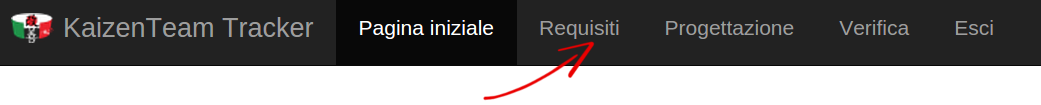
\includegraphics[width=\textwidth]{Pics/HomePageMenuFrecciaReq}
						\end{figure}
						\item Scegliere uno dei requisiti ai quali si intende associare un componente e cliccare sul pulsante “Modifica”.
						\begin{figure}[H]
							\centering
							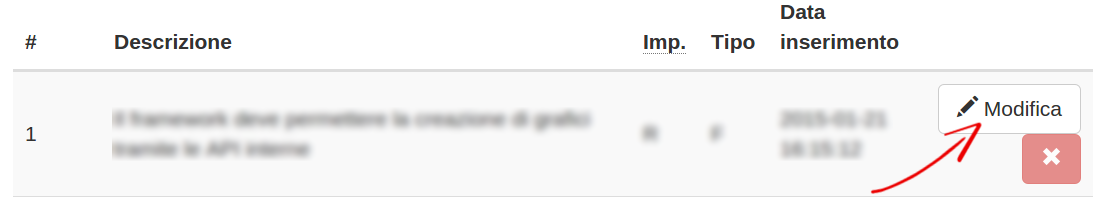
\includegraphics[width=\textwidth]{Pics/VistaRequisitoFrecciaModifica}
						\end{figure}
						\item Cercare la sezione “Componenti abbinati”. Scegliere dal menù a tendina il componente che realizza il requisito scelto al passo precedente. Cliccare sul pulsante “Aggiungi”. Un requisito  può essere associato a più componenti.
						\begin{figure}[H]
							\centering
							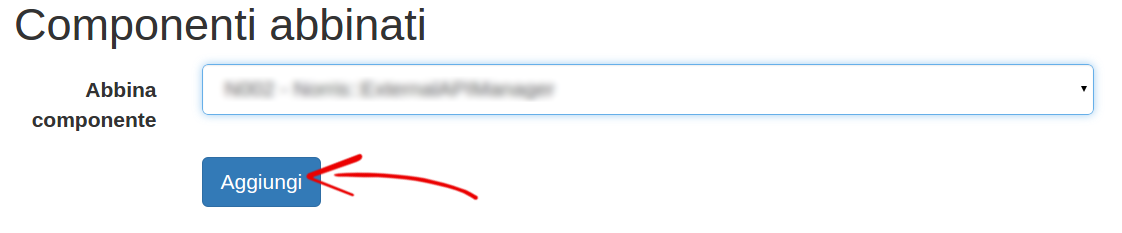
\includegraphics[width=\textwidth]{Pics/AbbianareComponenteRequisito}
						\end{figure}
						\item Eseguire il passo precedente per tutti i requisiti.
					\end{enumerate}
				\level{6}{Inserimento di un componente sul Tracker} \label{sec:InsComponente}
					Per poter effettuare correttamente i vari tracciamenti necessari si deve inserire all'interno del tracker del gruppo tutti i componenti che sono stati individuati dai \insrole{Progettisti} durante la progettazione architetturale. Per fare ciò si segua la seguente \insglo{procedura}.
					\begin{enumerate}
						\item Accedere al Kaizen \insglo{Team} Tracker (\insuri{http://kaizenteam.it/tracker/}).
						\item Entrare all'interno della sezione “Progettazione”.
						\begin{figure}[H]
							\centering
							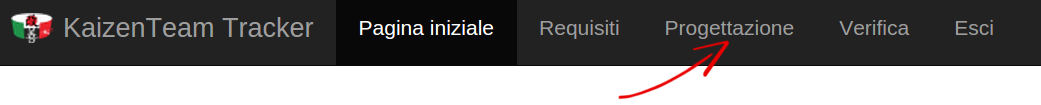
\includegraphics[width=\textwidth]{Pics/HomePageMenuFrecciaProg}
						\end{figure}
						\item Assicurarsi di essere all'interno della scheda “Componenti”.
						\item Cliccare sul pulsante “Aggiungi componente”.
						\item Inserire il codice del componente che si desidera aggiungere e una sua descrizione (secondo le norme presenti nella sezione \nameref{sec:ClassificareComponenti}). Cliccare in seguito su “Salva”.
						\begin{figure}[H]
							\centering
							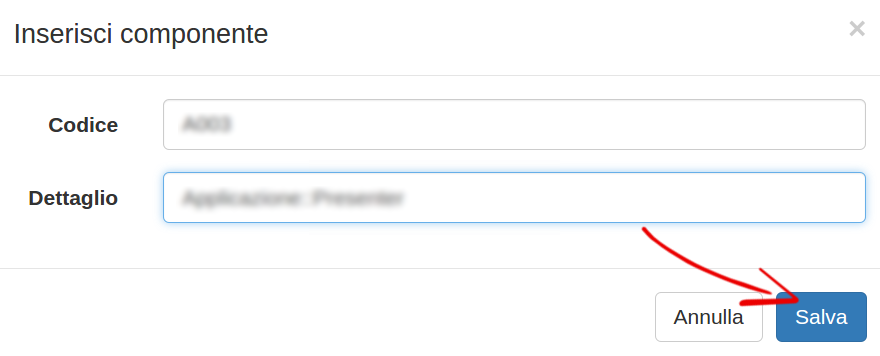
\includegraphics[width=\textwidth]{Pics/InserireComponente}
						\end{figure}
						\item Eseguire nuovamente i passi precedenti per inserire un nuovo componente all'interno del Tracker.
					\end{enumerate}

		\level{4}{Progettazione di dettaglio}
			Dopo che l'architettura del sistema è stata definita completamente, si può procedere alla progettazione di dettaglio. Essa prevede che vengano eseguiti e successivamente documentati i seguenti task:
			\begin{enumerate}
				\item si individuano le classi che implementano ciascuno dei componenti trovati durante la progettazione architetturale;
				\item si definiscono i ruoli e le responsabilità di ciascuna delle classi individuate;
				\item si definiscono le interazioni che le classi hanno fra di loro;
				\item ognuna delle classi deve essere definita nel dettaglio (vedi sezione \nameref{sec:DescrizioneClasse} per maggiori informazioni);
				\item ci si assicura che ogni requisito sia soddisfatto da almeno una delle classi individuate e descritte;
				\item ci si assicura che ogni classe realizzi almeno un requisito;
				\item si realizzano e si documentano i test di unità, necessari per verificare il corretto comportamento delle classi (le norme da seguire sono presenti nella sezione \nameref{sec:TestUnita}).
			\end{enumerate}
			Durante la suddivisione di un componente in classi è auspicabile che i \insrole{Progettisti} utilizzino in modo appropriato i \insglo{design pattern}. Qualora ciò dovesse avvenire, si documenta la cosa procedendo con una loro descrizione e contestualizzazione (per maggiori informazioni si consulti la sezione \nameref{sec:ProgDetDesingPattern}).\\
			Un utile supporto alla documentazione di tutti i task precedentemente descritti sono i diagrammi \insglo{UML}. Per maggiori informazioni si consulti la sezione \nameref{sec:ProgDetUML}.\\
			Il modo in cui viene effettuato il tracciamento dei requisiti viene descritto in modo più approfondito nella sezione \nameref{sec:ProgTracClasReq}.

			\level{5}{Norme}
				\level{6}{Design Pattern} \label{sec:ProgDetDesingPattern}
					Al fine di consentire una migliore comprensibilità  delle scelte progettuali e della progettazione di stessa, i \insrole{Progettisti} dovranno indicare i \insglo{pattern} impiegati, fornendo per ciascuno di essi:
					\begin{itemize}
						\item una descrizione testuale e grafica;
						\item la motivazione che ha portato alla sua scelta;
						\item una breve descrizione dell'applicazione del \insglo{pattern} al progetto.
					\end{itemize}
				\level{6}{Diagrammi UML} \label{sec:ProgDetUML}
					La documentazione riguardante le classi individuate deve sempre fare uso di diagrammi \insglo{UML}. Essi sono necessari per esplicitare e formalizzare in modo migliore i vari aspetti che sono stati descritti testualmente.\\
					In particolare, durante la progettazione di dettaglio è necessario fare uso dei seguenti diagrammi:
					\begin{description}
						\item[diagrammi delle classi] Essi hanno lo scopo di descrivere \texttt{tipi di entità}, con le loro caratteristiche ed eventuali relazioni fra questi tipi. Questo tipo di diagramma viene utilizzato per evidenziare e descrivere in modo dettagliato le classi e le relazioni che esistono tra di loro.
						\item[diagrammi delle attività] Essi hanno lo scopo di definire le attività da svolgere per realizzare una certa funzionalità. Vengono dunque usati per mostrare come determinate interazioni tra classi realizzino una funzionalità che si intende rendere disponibile.
						\item[diagrammi di sequenza] Essi hanno lo scopo di descrivere scenari (determinate sequenze di azioni in cui tutte le scelte sono già state effettuate). Vengono usati per descrivere le relazioni che intercorrono, in termini di messaggi, tra attori, oggetti ed entità del sistema che si sta rappresentando.
					\end{description}
					Tali diagrammi dovranno seguire le indicazioni fornite nella sezione \nameref{sec:UML}.
				\level{6}{Classificazione delle classi} \label{sec:ClassificareClassi}
					Le classi vengono identificate univocamente da una descrizione nella forma\\ NomeProdotto::NomeComponente::NomeClasse.
					\begin{itemize}
						\item NomeProdotto rappresenta il nome del \insglo{prodotto} \insglo{software} che i \insrole{Progettisti} hanno deciso di realizzare.
						\item NomeComponente rappresenta il nome che è stato dato dai \insrole{Progettisti} al componente al quale appartiene la classe.
						\item NomeClasse rappresenta il nome che è stato dato dai \insrole{Progettisti} alla classe individuata.
					\end{itemize}
					A ogni classe è inoltre associato un codice univoco nella forma XY, dove X è l'iniziale del del nome del \insglo{prodotto} e Y un numero intero crescente (che parte da 0).\\
				\level{6}{Descrivere le classi} \label{sec:DescrizioneClasse}
					Per descrivere in modo completo una classe, i \insrole{Progettisti} devono preoccuparsi di individuare e descrivere:
					\begin{itemize}
						\item il nome;
						\item la visibilità;
						\item gli attributi;
						\item i metodi.
					\end{itemize}
					È inoltre necessaria una descrizione generica che indichi lo scopo e le responsabilità della classe in questione. Infine, devono essere descritte dettagliatamente (anche mediante l'uso di appropriati diagrammi) le relazioni con altre classi e le interfacce che mette a disposizione.
				\level{6}{Test di unità} \label{sec:TestUnita}
					Durante la definizione dei test di unità necessari per verificare che il funzionamento delle classi sia quello previsto, i \insrole{Progettisti} devono preoccuparsi di rispettare la seguente regola: colui o colei che progetta il test deve necessariamente essere una persona diversa da quella che ha progettato e descritto nel dettaglio la classe in questione.

			\level{5}{Strumenti}
				Per la progettazione di dettaglio è stato utilizzato il \insglo{software} \insglo{Astah}, descritto nell'appendice \nameref{app:strumenti}, per la creazione dei diagrammi \insglo{UML}.

			\level{5}{Procedure}
				\level{6}{Tracciamento classi-requisiti} \label{sec:ProgTracClasReq}
					È fondamentale che ogni requisito sia soddisfatto da almeno una classe. Per controllare che ciò sia vero è necessario prima di tutto effettuare il tracciamento. Si seguano i passi descritti nella seguente \insglo{procedura}. Si noti che qui si da per scontato che le classi e i requisiti siano già stati inseriti precedentemente sul Tracker del gruppo (per l'inserimento delle classi fare riferimento alla \insglo{procedura} descritta nella sezione \nameref{sec:InsClasse}).
					\begin{enumerate}
						\item Accedere al Kaizen \insglo{Team} Tracker (\insuri{http://kaizenteam.it/tracker/}).
						\item Entrare all'interno della sezione “Requisiti”.
						\begin{figure}[H]
							\centering
							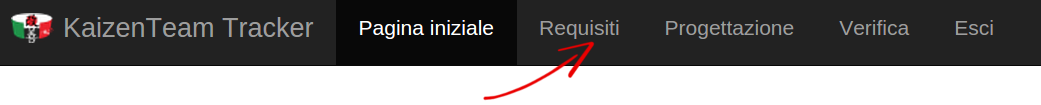
\includegraphics[width=\textwidth]{Pics/HomePageMenuFrecciaReq}
						\end{figure}
						\item Scegliere uno dei requisiti ai quali si intende associare una classe e cliccare sul pulsante “Modifica”.
						\begin{figure}[H]
							\centering
							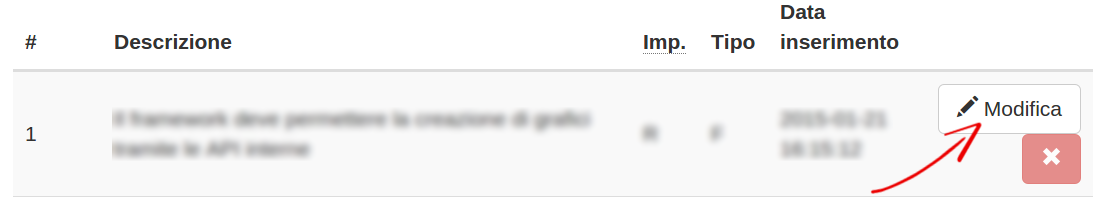
\includegraphics[width=\textwidth]{Pics/VistaRequisitoFrecciaModifica}
						\end{figure}
						\item Cercare la sezione “Classi abbinate”. Scegliere dal menù a tendina la classe che realizza il requisito scelto al passo precedente. Cliccare sul pulsante “Aggiungi”. Un requisito  può essere associato a più classi.
						\begin{figure}[H]
							\centering
							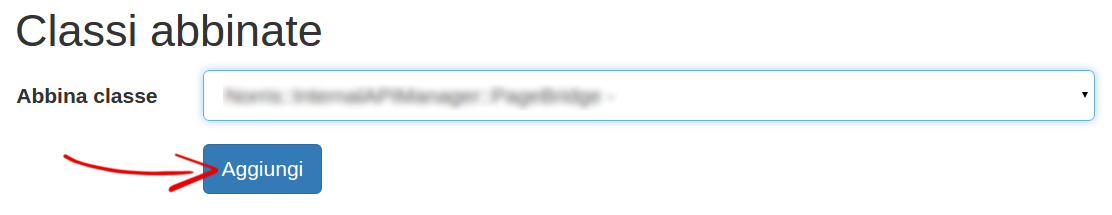
\includegraphics[width=\textwidth]{Pics/AbbinareClasseRequisito}
						\end{figure}
						\item Eseguire il passo precedente per tutti i requisiti.
					\end{enumerate}
				\level{6}{Inserimento di una classe sul Tracker} \label{sec:InsClasse}
					Per poter effettuare correttamente i vari tracciamenti necessari si deve inserire all'interno del tracker del gruppo tutti le classi che sono state individuate dai \insrole{Progettisti} durante la progettazione di dettaglio. Per fare ciò si segua la seguente \insglo{procedura}.
					\begin{enumerate}
						\item Accedere al Kaizen \insglo{Team} Tracker (\insuri{http://kaizenteam.it/tracker/}).
						\item Entrare all'interno della sezione “Progettazione”.
						\begin{figure}[H]
							\centering
							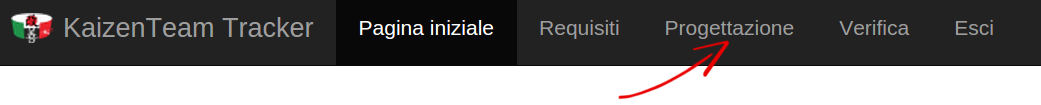
\includegraphics[width=\textwidth]{Pics/HomePageMenuFrecciaProg}
						\end{figure}
						\item Assicurarsi di essere all'interno della scheda “Classi”.
						\item Cliccare sul pulsante “Aggiungi classe”.
						\item Inserire il codice della classe che si desidera aggiungere e una sua descrizione (secondo le norme presenti nella sezione \nameref{sec:ClassificareClassi}). Cliccare in seguito su “Salva”.
						\begin{figure}[H]
							\centering
							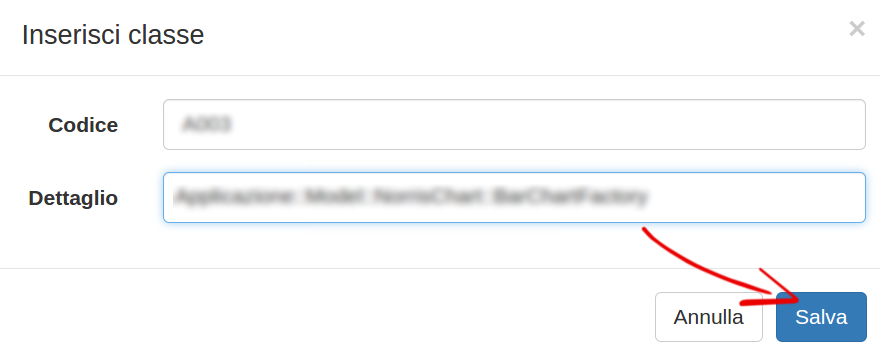
\includegraphics[width=\textwidth]{Pics/InserireClasse}
						\end{figure}
						\item Eseguire nuovamente i passi precedenti per inserire un nuovo componente all'interno del Tracker.
					\end{enumerate}

	\level{3}{Codifica} \label{sec:codifica}
		L'attività di codifica ha lo scopo di produrre il codice necessario alla realizzazione del \insglo{prodotto} richiesto. Il codice generato dovrà rispettare il più fedelmente possibile ciò che è stato definito nel documento \insdoc{Definizione di Prodotto v1.00}.\\
		L'attività di codifica, in generale, prevede che siano svolti i seguenti task:
		\begin{enumerate}
			\item codifica di ciascuna unità identificata e descritta durante la progettazione di dettaglio;
			\item scrittura della documentazione riguardante la codifica del punto precedente.
		\end{enumerate}
		Durante l'esecuzione dei task precedentemente citati si devono rispettare determinate norme. In particolare, quando si codifica utilizzando un certo linguaggio si devono rispettare le convenzioni che sono state fissate (consultare la sezione \nameref{sec:LineeGuida}).\\
		Ogni file, inoltre, deve possedere un'intestazione nel formato corretto (vedi \nameref{sec:CodificaIntestazione}).\\
		Infine, ulteriori regole generali da seguire durante l'attività di codifica sono riportate in \nameref{sec:CodificaNormeGenerali}.
		\level{4}{Norme}
			\level{5}{Regole generali da seguire durante la codifica di un file} \label{sec:CodificaNormeGenerali}
				Durante la codifica di un file si devono rispettare alcune regole generali:
				\begin{itemize}
					\item l'indentazione del codice deve essere di quattro spazi;
					\item le righe non devono essere più lunghe di 80 caratteri.
				\end{itemize}
				Inoltre, ogniqualvolta la difficoltà di certi passaggi lo richieda, il programmatore è tenuto a commentare il codice da lui scritto. Per quanto riguarda le norme da seguire per la stesura dei commenti, si consulti la sezione \nameref{sec:NormeCommenti}. 
				Infine, tutti i file di codice devono seguire quanto riportato nella sezione \nameref{sec:CodificaFile}.
			\level{5}{Linee guida all'utilizzo dei linguaggi di programmazione} \label{sec:LineeGuida}
				Nel corso del progetto vengono utilizzati alcuni linguaggi di programmazione. Quando si utilizza uno di essi si devono rispettare alcune regole, in modo tale da favorire nel maggior modo possibile la comprensibilità del codice. Si cerca, dove possibile, di adottare linee guida accettate a livello internazionale.\\
				In seguito, per ogni linguaggio adottato, viene indicata una sorgente alla quale è possibile trovare le linee guida da seguire.
				\begin{description}
					\item[\insglo{JavaScript}] Quando si fa uso di questo linguaggio di programmazione si deve rispettare quanto riportato all'indirizzo \insuri{https://google-styleguide.googlecode.com/svn/trunk/javascriptguide.xml}.
					\item[\insglo{Java}] Quando si fa uso di questo linguaggio di programmazione si deve rispettare quanto riportato all'indirizzo \insuri{https://google-styleguide.googlecode.com/svn/trunk/javaguide.html}
				\end{description}
			\level{5}{Intestazione dei file} \label{sec:CodificaIntestazione}
				Ogni file \insglo{prodotto} durante l'attività di codifica (a prescindere dal linguaggio di programmazione usato) deve iniziare con un'intestazione che rifletta la seguente struttura:
				\begin{lstlisting}
					/*
					* Name: [nome del file]
					* (*\ignoreglo{Package}*): [(*\ignoreglo{package}*) al quale appartiene il file]
					* Location: [path della directory di appartenenza]
					* Date: [data di creazione del file]
					* Version: [versione del file]
					* 
					* History:
					* 
					* =================================================================
					* Version  Date        Programmer    Changes
					* =================================================================
					* v0.01    AAAA-MM-GG  Nome Cognome  {descrizione modifica}
					* =================================================================
					*
					*/
				\end{lstlisting}
				dove:
				\begin{description}
					\item[Name] indica il nome del file comprensivo di estensione;
					\item[\ignoreglo{Package}] indica il \insglo{package} al quale appartiene il file, comprensivo di gerarchia;
					\item[Location] indica il path della directory in cui è presente il file;
					\item[Date] indica la data di creazione del file: si veda la sezione \nameref{sec:formatoDate} per il formato da utilizzare;
					\item[Version] indica l'attuale versione del codice, il cui formato da seguire è descritto nella sezione \nameref{sec:versioni};
					\item[History] visualizza lo storico delle modifiche del file in questione, comprensive di versione, data, descrizione e nome del programmatore che ha modificato il codice.
				\end{description}
			\level{5}{Commenti} \label{sec:NormeCommenti}
			Allo scopo di mantenere ordinato e leggibile il codice, è necessario commentarlo nel modo più appropriato. In questo modo, il codice risulterà più comprensibile, non solo per gli altri membri del \insglo{team} e per il programmatore stesso, ma anche per i fruitori esterni che utilizzeranno il \insglo{prodotto}. In questo modo sarà facilitato il riuso del codice e la sua leggibilità. \\
			I commenti devono essere tassativamente in lingua inglese, significativi e determinanti per la corretta comprensione e per l'interpretazione del codice scritto.\\
			Al fine di usufruire della generazione automatica della documentazione del codice, grazie a strumenti specifici, come \insglo{JSDOC} e \insglo{JAVADOC}, è fondamentale l'utilizzo di una precisa sintassi per la scrittura dei commenti.
			Di seguito, si elencano le norme da seguire a seconda del linguaggio di programmazione adottato.
			\begin{description}
					\item[\insglo{JavaScript}] I commenti devono rispettare la seguente struttura:
						\begin{itemize}
							\item Prima di ogni dichiarazione di classe deve essere scritto un commento che deve cominciare con i simboli “/**”, deve avere, all'inizio di ogni riga “*” e deve terminare con “*/” (particolare forma di commento multi-linea). Esso deve riflettere la seguente struttura:
							\begin{lstlisting} 
								/**
								* Creates a new NomeClasse. 
								* @constructor
								* @param {tipoParametro} Descrizione del parametro 
								*/
								function NomeClasse(listaParametri){}
							\end{lstlisting}
							Si fa presente che “@param” deve essere ripetuto per ogni parametro della lista dei parametri, ciascuno in una riga diversa e successiva alla precedente (in caso non ci siano parametri questa riga non va scritta).\\
							Si noti che il tipo del parametro deve essere scritto tra parentesi graffe.
							\item Prima di ogni metodo deve essere scritto un commento che rispetti la seguente struttura:
							\begin{lstlisting} 
								/**
								* Descrizione del metodo 
								* @param {tipoParametro} nomeParametro Descrizione del parametro
								* @return {tipoDiRitorno} Descrizione 
								*/
								public tipoDiRitorno nomeMetodo(listaParametri){}
							\end{lstlisting}
							Si noti che anche per i commenti che precedono i metodi si devono utilizzare i simboli descritti per quelli che precedono le classi (“/**”, “*”, “*/”). Inoltre, si seguano le stesse regole, descritte nel punto precedente per “@param”. Infine, “@return” deve essere specificato solo quando viene effettivamente ritornato qualcosa. \\
							Anche in questo caso, si fa presente che il tipo del parametro e il tipo di ritorno devono essere racchiusi tra parentesi graffe.
						\end{itemize}
					\item[\insglo{Java}] I commenti devono rispettare la seguente struttura:
						\begin{itemize}
							\item Prima di ogni dichiarazione di classe deve essere scritto un commento che ne descriva la funzionalità e lo scopo. Esso deve cominciare con i simboli “/**”, deve avere, all'inizio di ogni riga “*” e deve terminare con “*/” (particolare forma di commento multi-linea).
							\begin{lstlisting}
								/**
								* Descrizione della classe
								*/
								public class NomeClasse(){}
							\end{lstlisting}
							\item Prima di ogni metodo deve essere scritto un commento che rispetti la seguente struttura:
							\begin{lstlisting}
								/**
								* Descrizione del metodo
								* @param nomeParametro Descrizione del parametro 
								* @return tipoDiRitorno Descrizione 
								*/
								public tipoDiRitorno nomeMetodo(lista parametri){}
							\end{lstlisting}
							Si noti che anche per i commenti che precedono i metodi si devono utilizzare i simboli descritti per quelli che precedono le classi (“/**”, “*”, “*/”). Inoltre, “@param” deve essere ripetuto per ogni parametro della lista dei parametri del metodo, ciascuno in una riga diversa e successiva alla precedente (in caso non ci siano parametri questa riga non va scritta). Infine, “@return” deve essere specificato solo quando il tipo di ritorno del metodo non è “void”.
						\end{itemize}
			\end{description}
		\level{4}{Strumenti}
			Per la scrittura di codice \insglo{JavaScript} non è richiesto l'utilizzo di un particolare \insglo{IDE}; la scelta dell'editor di testo è affidata alla discrezione dello sviluppatore.\\
			Per lo sviluppo dell'applicazione \insglo{Android} si utilizza l'\insglo{IDE} \ignoreglo{Android} Studio, descritto nell'appendice \nameref{app:strumenti} del presente documento.